\documentclass[c,aspectratio=169]{beamer}
\setbeamertemplate{navigation symbols}{}%remove navigation symbols
\usepackage[utf8]{inputenc}
\usepackage{multimedia}
\DeclareUnicodeCharacter{20AC}{\euro{}} % L'euro, oublié par inputenc…
\usepackage[T1]{fontenc} % Encodage de sortie
\usepackage{graphics}
\usepackage[absolute,overlay]{textpos}
\usepackage{caption}
\usepackage{hyperref}
\usepackage{minted}
\definecolor{dgreen}{rgb}{0.,0.6,0.}
\usetheme{Warsaw}
\useoutertheme{infolines}
\title[mc\_rtc logging: beyond visualization]{mc\_rtc logging: beyond visualization}
\author[\rmfamily P. \textsc{Gergondet}]{\rmfamily Pierre \textsc{Gergondet}}
\date{\rmfamily 2021-10-29}

\begin{document}

{
\setbeamertemplate{headline}{}
\begin{frame}
  \titlepage
  \begin{center}
    \vspace{-6.5em}
    \rmfamily Beijing Institute of Technology, \textsc{China}

    \vspace{4em}

    Code and presentation available online

    \hyperlink{https://github.com/gergondet/mc-rtc-tutorial-logging}{github.com/gergondet/mc-rtc-tutorial-logging}
  \end{center}
\end{frame}

\begin{frame}<beamer>
  \frametitle{Presentation layout}
  \setcounter{tocdepth}{1}
  \tableofcontents
\end{frame}
} % Ends no headline

\section{Back to basics}

\begin{frame}<beamer>
  \frametitle{Presentation layout}
  \setcounter{tocdepth}{2}
  \tableofcontents[currentsection,hideothersubsections]
\end{frame}

\subsection{Adding/Removing data to/from the log}

\begin{frame}[fragile]{Basics}

  \begin{block}{Add and remove data}

\scriptsize
\begin{minted}{cpp}
  // In every sample in this presentation logger is a mc_rtc::Logger

  logger.addLogEntry("name", []() { return data; });

  logger.removeLogEntry("name");
\end{minted}

  \end{block}

  \begin{block}{Add data but avoid copy}

\scriptsize
\begin{minted}{cpp}
  logger.addLogEntry("name", []() -> const Eigen::Vector3d & { return data; });
\end{minted}

  \end{block}

\end{frame}

\begin{frame}[fragile]{Basics++}

  \vspace{-0.5em}
\scriptsize
  \begin{block}{Add data with a source}

\begin{minted}{cpp}
  logger.addLogEntry("a", this, [this]() { return a_; });
  logger.addLogEntry("b", this, [this]() { return b(); });

  // OR

  logger.addLogEntries(this,
                       "a", [this]() { return a_; },
                       "b", [this]() { return b(); });

  // OR (automatically avoid copies)

  MC_RTC_LOG_HELPER("a", a_);
  // expands to: logger.addLogEntry<decltype(&ThisClass::a_), &ThisClass::a_>("a", this)
  // i.e. logger.addLogEntry("a", this, [this] -> const decltype(a_) & { return a_; })
  MC_RTC_LOG_GETTER("b", b);

  // Remove everything added by this
  logger.removeLogEntries(this);

\end{minted}

  \end{block}

\end{frame}

\begin{frame}[fragile]{What can go in a log?}

  \begin{itemize}
    \item Numeric types: \verb|bool|, \verb@[u]int[8|16|32|64]_t@, \verb|float|, \verb|double|;
    \item Strings: \verb|std::string|;
    \item STL containers: \verb|std::vector<double>|, \verb|std::array<double, N>|;
    \item Eigen types: \verb|Quaterniond|, \verb@Vector[2|3|6|X]d@, \verb|Ref|;
    \item SVA types: \verb|PTransformd|, \verb|MotionVecd|, \verb|ForceVecd|, \verb|ImpedanceVecd|;
  \end{itemize}

  \bigskip

  The log contains data identifying the type so it can be used in log tools.

  \medskip

  The type of an entry can change throughout the life of the program and it's ok.

  \medskip

  Dynamically sized entries can change size as well.

\end{frame}

\subsection{Graphic tools}

\begin{frame}{mc\_log\_ui}

  \centering
  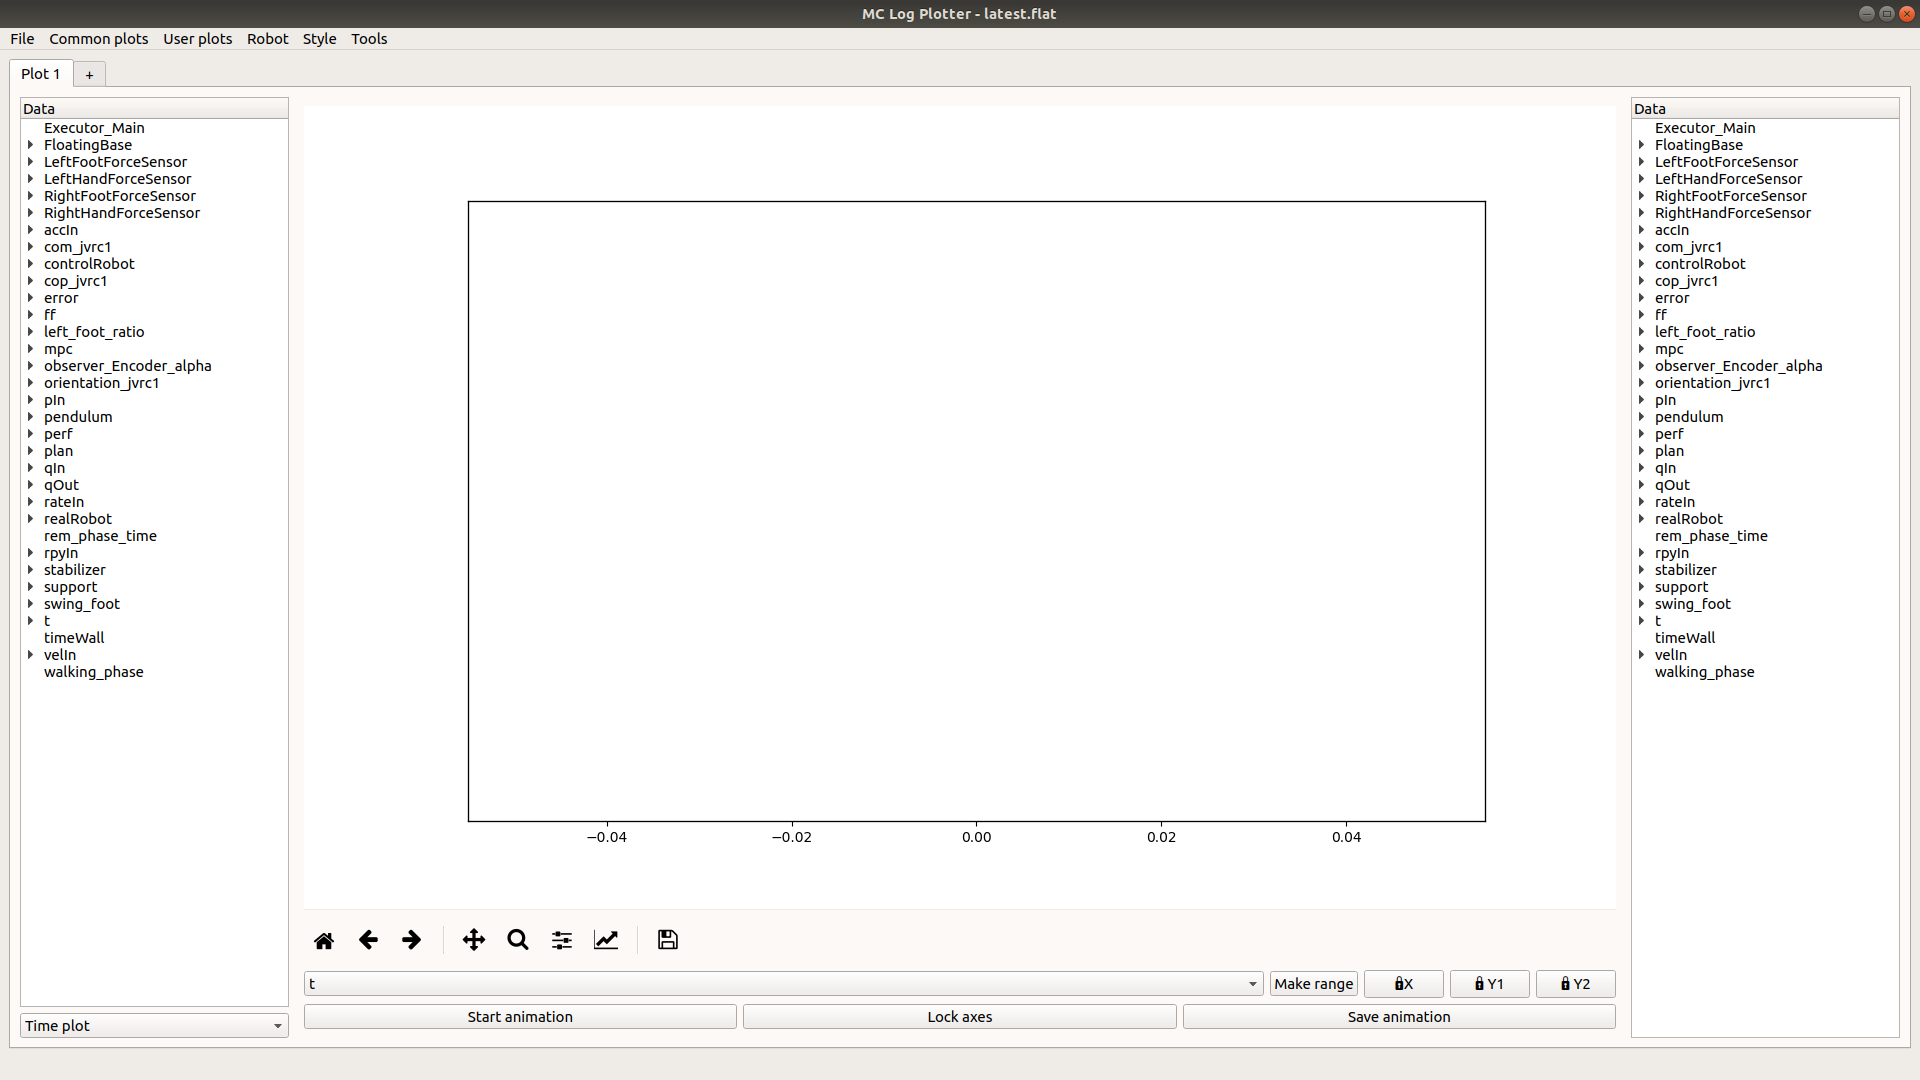
\includegraphics[width=0.7\textwidth]{img/mc_log_ui.png}

\end{frame}

\begin{frame}[fragile]{mc\_log\_ui: ``User plots''}
  Let you save the current plot, i.e.:
  \begin{itemize}
    \item Selected data
    \item Plot style, color, legends, labels
  \end{itemize}

  \vfill

  The plot can be restored with any log file -- missing data is ignored.

  \vfill

  All plots are saved in \verb|$HOME/.config/mc_log_ui/custom_plot.json|

\end{frame}

\begin{frame}[fragile]{mc\_log\_ui: lesser known features}

  Open multiple logs at once: \verb|mc_log_ui log-1.bin log-2.bin ... log-N.bin|

  \vfill

  Generate figures from a log: \verb|mc_plot_logs log.bin custom_plot.json|

  \vfill

  Open the log in Python

  \scriptsize
  \begin{minted}{Python}
    import mc_log_ui
    log = mc_log_ui.read_log('log.bin')

    # log is a dictionnary:
    # - the key is what you see in mc_log_ui (e.g. CoM_target_x)
    # - the data is a numpy array (with NaN when the data is absent)

  \end{minted}
\end{frame}

\begin{frame}[fragile]{mc\_log\_visualization}
  Start with: \scriptsize \verb|roslaunch mc_log_visualization log_visualizer.launch robot:=JVRC1 log:=/tmp/my-log.bin|

  \begin{center}
    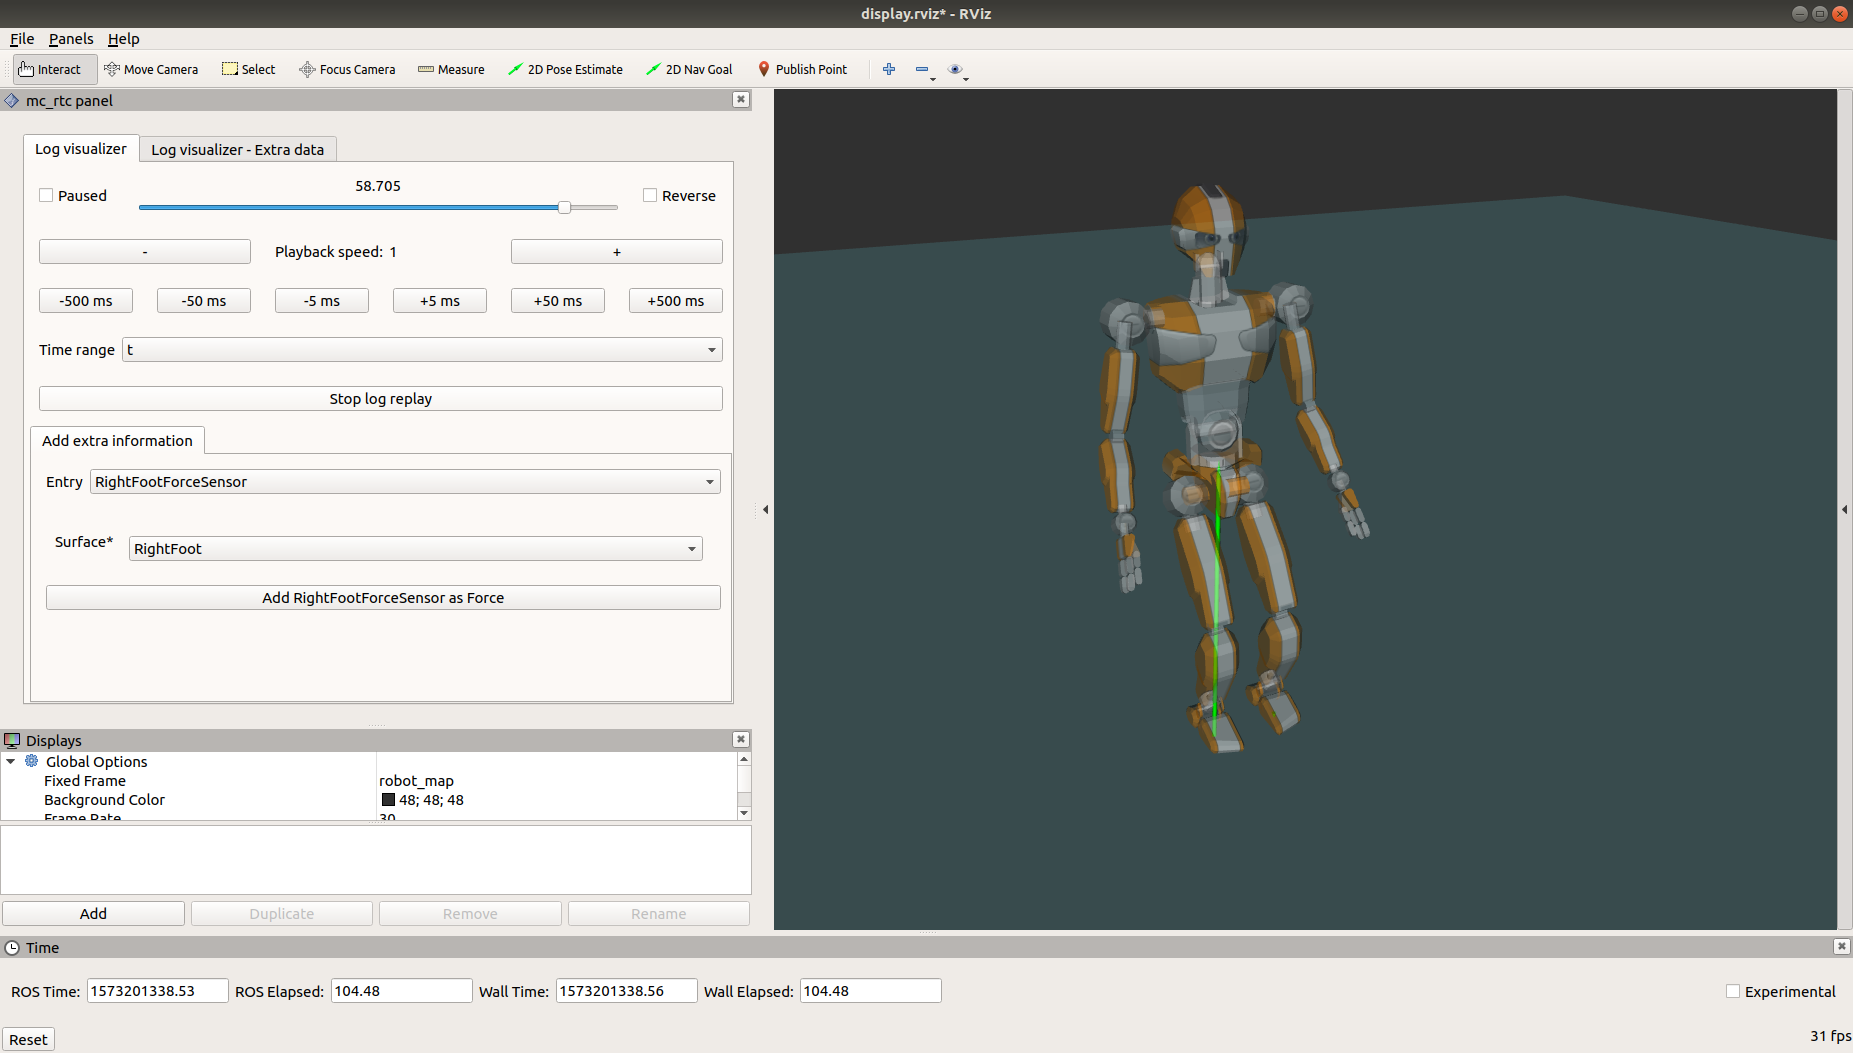
\includegraphics[width=0.5\textwidth]{img/mc_log_visualization.png}
  \end{center}
\end{frame}

\subsection{Command lines tools}

\begin{frame}[fragile]{Conversion utilities: mc\_bin\_to\_*}
  Convert \verb|.bin| files to another format

  \medskip

  \begin{description}
    \item[mc\_bin\_to\_log] \hfill \\ Convert a \verb|.bin| file to a \verb|.csv| file
    \item[mc\_bin\_to\_rosbag] \hfill \\ Convert a \verb|.bin| file to a \verb|.rosbag| file
    \item[mc\_bin\_to\_flat] \hfill \\ Convert a \verb|.bin| file to a \verb|.flat| file
  \end{description}
\end{frame}

\begin{frame}[fragile]{Performance at a glance: mc\_bin\_perf}

  Extract \verb|Perf_*| entries from a log and shows some statistics

  \scriptsize

  \begin{minted}{text}
    > mc_bin_perf /tmp/mc-control-CoM-latest.bin
    ----------------------------------------------------------------
    |                     |  Average |    StdEv |      Min |   Max |
    ----------------------------------------------------------------
    |       ControllerRun |    0.451 |   0.0639 |    0.378 |  1.14 |
    |       FrameworkCost |     7.64 |     2.81 |     2.55 |  52.8 |
    |           GlobalRun |    0.488 |   0.0703 |    0.401 |  1.18 |
    |                 Gui |   0.0035 |  0.00941 | 0.000543 | 0.322 |
    |                 Log |  0.00732 |  0.00476 |  0.00563 | 0.163 |
    |        ObserversRun | 6.79e-05 | 0.000215 |  2.4e-05 | 0.014 |
    |   Plugins_ROS_after |   0.0137 |   0.0124 |  0.00202 | 0.172 |
    | SolverBuildAndSolve |    0.422 |   0.0607 |    0.354 |  1.11 |
    |         SolverSolve |     0.32 |   0.0498 |    0.268 |     1 |
    ----------------------------------------------------------------
  \end{minted}

  \normalsize

  This works with your own \verb|Perf_*| entries
\end{frame}

\begin{frame}[fragile]{General utility: mc\_bin\_utils}

  \verb|mc_bin_utils [command] (options) [log.bin]| where \verb|command| is:

  \begin{description}
    \item[show] \hfill \\ Show general information about the log content
    \item[split] \hfill \\ Split a long in multiple parts
    \item[convert] \hfill \\ Forward to the right \verb|mc_bin_to_*|
    \item[extract] \hfill \\ Extract part of a log
  \end{description}

  \scriptsize
  \begin{minted}{bash}
    # Extract the part of a log where the provided key is present
    mc_bin_utils extract log.bin log_out --key com_target
    # Extract the specified time range from the log (50s to 100s here)
    mc_bin_utils extract log.bin log_out --from 50 --to 100
  \end{minted}
\end{frame}

\section{Advanced manipulations with FlatLog}

\begin{frame}<beamer>
  \frametitle{Presentation layout}
  \setcounter{tocdepth}{1}
  \tableofcontents[currentsection,hideothersubsections]
\end{frame}

\begin{frame}{Context and objective}
  In this tutorial we will use a simple controller with three tasks:
  \begin{enumerate}
    \item Floating base task to control the robot attitude;
    \item Left hand task;
    \item Right hand task;
  \end{enumerate}

  These tasks are controlled via a joystick with the following controls:
  \begin{description}
    \item[L1/R1] Change the ``active'' task;
    \item[Analog] Move/Rotate along/around X|Y|Z axis;;
    \item[L2] While pushed the sticks control the rotation;
    \item[R2] While pushed changes the default transformation frame (local for rotation, global for translation);
  \end{description}

  We want to record and replay these inputs and we want it to be relatively transparent.
\end{frame}

\begin{frame}<beamer>
  \frametitle{Presentation layout}
  \setcounter{tocdepth}{2}
  \tableofcontents[currentsection,hideothersubsections]
\end{frame}

\begin{frame}[fragile]{Step 0: controller structure}
  Simple FSM with three states: \verb|Initial|, \verb|Joystick::Live| and \verb|Joystick::Replay|

  \medskip

  \verb|Joystick::Live| and \verb|Joystick::Replay| based on the same C++ state: \verb|Joystick|

  \vfill

  The \verb|Joystick| plugin provides a \verb|mc_joystick::State| reading

  \medskip

  We will mimic this input by reading the recording from a log


\end{frame}


\subsection{Step 1: record the inputs}
\begin{frame}[fragile]{Recording the inputs}
  \begin{block}{Our Joystick state is available as \texttt{current\_state\_}}

  \scriptsize
  \begin{minted}{cpp}
    // Joystick::start(ctl)
    logger.addLogEntry("L1", this, [this] -> bool { return s.buttons[Button::L1]; });
    // ...
    logger.addLogEntry("Left_LR", this, [this] -> double { return s.axes[Axis::Left_LR]; });

    // Joystick::teardown(ctl)
    logger.removeLogEntries(this);
  \end{minted}
  \end{block}

  \bigskip

  \hfill To fit in the slide, assume:
  \begin{itemize} \raggedleft
    \item \verb|#define s current_state_|
    \item All entries are prefixed with \verb|Joystick_|
  \end{itemize}
\end{frame}

\subsection{Step 2: make it transparent}
\begin{frame}[fragile]{Make it transparent: initial state}
  \begin{block}{We build an initial state where the user can choose to use a live joystick or replay a log}

  \scriptsize
  \begin{minted}{cpp}
    // Initial::reset(ctl)
    ctl.gui()->addElement({},
                          Button("Live", [this]() { output("Live"); }),
                          Button("Replay", [this]() { output("Replay"); }));

    // Initial::run(ctl)
    return !output().empty();

    // Initial::teardown(ctl)
    // GUI cleanup
  \end{minted}
  \end{block}

  \scriptsize
  \hfill For the sake of simplicity we do not give a choice of replay log.

  \normalsize

  \begin{block}{This goes with the transition map}
  \scriptsize
  \begin{minted}{yaml}
    transitions:
    - [Initial, Live, Joystick::Live, Auto]
    - [Initial, Replay, Joystic::Replay, Auto]
  \end{minted}
  \end{block}

\end{frame}

\begin{frame}[fragile]{Make it transparent: joystick state}
  \scriptsize
  \begin{block}{We build a callback to get the joytstick state based on the source}
  \begin{minted}{cpp}
    // Joystick::start(ctl)
    if(source == "Live") {
      callback = [this](mc_control::fsm::Controller & ctl) {
        current_state_ = *ctl.datastore().get<const mc_joystick::State *>(joystick_);
      };
    } else {
      // Load the log (ideally async load from the initial state)
      callback = [this](mc_control::fsm::Controller &) {}; // TODO
    }

    // Joystick::run(ctl)
    update_state(ctl);
    // Deal with the joystick input

    // Joystick::update_state(ctl)
    previous_state_ = current_state_;
    callback(ctl);
  \end{minted}
  \end{block}
\end{frame}

\subsection{Step 3: replay the inputs}
\begin{frame}[fragile]{Binary log format and flat log}

  Format of the binary log:

  \verb@mc_rtc::Logger::magic [([keys]|null), [type, data]][N]@

  \vfill

  For most manipulations the following is more interesting and efficient:

  \verb@key: [type, data][N]@

  \vfill

  This is the flat format, we have two tools to exploit it:
  \begin{description}
    \item [mc\_rtc::log::FlatLog] \hfill \\ Provides a C++ view over this transformation
    \item [mc\_bin\_to\_flat] \hfill \\ Strip the type information for efficient loading in mc\_log\_ui
  \end{description}

\end{frame}

\begin{frame}[fragile]{mc\_rtc::log::FlatLog -- API}

  \scriptsize
  \begin{block}{}
    \begin{minted}{cpp}
// Load a binary file into a FlatLog
mc_rtc::log::FlatLog flat("log.bin");

// Number of entries in the log
size_t n_entries = flat.size();

// All entries in the log
std::set<std::string> entries = flat.entries();

// Check for existence of an entry
bool has_com = flat.has("CoM");

// Check the types of an entry
std::set<LogType> com_types = flat.types("CoM");

// First non null type (usually one entry has one type)
LogType com_type = flat.type("CoM");
    \end{minted}
  \end{block}

\end{frame}

\begin{frame}[fragile]{mc\_rtc::log::FlatLog -- Data API}

  \scriptsize
  \begin{block}{}
    \begin{minted}{cpp}
// Get raw value (pointer) for a given entry at a given index i, nullptr if:
// - the key was not recorded at time i
// - the key was recorded with a different type
const std::vector<double> * qIn_i = flat.getRaw<std::vector<double>>("qIn", i);

// Access all raw values
std::vector<const Eigen::Vector3d *> com = flat.getRaw<Eigen::Vector3d>("CoM_target");

// Value at index i, uses the default you provide for nullptr
sva::MotionVecd lf_vel_i = flat.get("LeftFootVel", i, sva::MotionVecd::Zero());

// Gives all values, uses the default you provide for nullptr
std::vector<double> stiffness = flat.get("t_stiffness", nan);

// Gives all values and fill the gap with first/last non null
std::vector<sva::ForceVecd> lf_s = flat.get<sva::ForceVecd>("LeftFootForceSensor");
    \end{minted}
  \end{block}

  \vfill

  \hfill Performance wise: \verb|raw[i] > value[i] > raws > values w/ default > values|

\end{frame}

\begin{frame}[fragile]{mc\_rtc::log::FlatLog -- Complete example}

  \begin{block}{Find the max normal force on a sensor during an experiment}
    \scriptsize
    \begin{minted}{cpp}
mc_rtc::log::FlatLog log("log.bin");
double max_force = 0.0;
for(size_t i = 0; i < log.size(); ++i)
{
  auto wrench = log.getRaw<sva::ForceVecd>("ForceSensor", i);
  if(!wrench)
  {
    continue;
  }
  max_force = std::max(std::fabs(wrench->linear().z()), max_force);
}
mc_rtc::log::info("Max force: {}", max_force);
    \end{minted}
  \end{block}

  Build your own tool to extract key indicators in your controller/observer.

\end{frame}

\begin{frame}[fragile]{Playback of the inputs}
  \begin{block}{Now we should be able to figure how to write our callback}
    \scriptsize
    \begin{minted}{cpp}
      // Load the log (ideally async load from the initial state)
      // Find the first index where data appear, store in log_idx
      callback = [this](mc_control::fsm::Controller &) {
        if(log_idx < log.size())
        {
          auto L1 = log.getRaw<bool>("L1");
          if(!L1) // end of log section
          {
            return;
          }
          current_state_.buttons[Button::L1] = *L1;
          // Rince and repeat for required buttons/axes
          log_idx++;
        }
      };
    \end{minted}
  \end{block}
\end{frame}

\begin{frame}{In action}
\end{frame}

\section{Drawbacks and alternate solutions}

\begin{frame}<beamer>
  \frametitle{Presentation layout}
  \setcounter{tocdepth}{2}
  \tableofcontents[currentsection,hideothersubsections]
\end{frame}

\subsection{Looking for a needle in a haystack}

\begin{frame}[fragile]{Solution 1: preprocess the log}
  \scriptsize
  \begin{minted}{bash}
    > mc_bin_utils extract log.bin joystick --key Joystick_L1
  \end{minted}

  \vfill

  \normalsize

  We're done... \pause but we did not learn anything new :)
\end{frame}

\begin{frame}[fragile]{Solution 2: recording a new log}
  \begin{block}{Create a separate log just for the joystick inputs}
    \scriptsize
    \begin{minted}{cpp}
      // Header
      mc_rtc::Logger logger = {mc_rtc::Logger::Policy::THREADED, "/tmp", "mc-joystick"};

      // start(ctl)
      logger.start("Joystick", ctl.solver().dt());
      // Use this logger instead of ctl.logger()

      // run(ctl) (after the state update)
      logger.log();
    \end{minted}
  \end{block}
  \vfill
  \verb|/tmp/mc-joystick-Joystick-latest.bin| now contains the inputs (and t) only
\end{frame}

\subsection{Eliminate the boilerplate}
\begin{frame}[fragile]{Towards more transparent inputs}
  Put everything we learned today and implement a ``log'' source for the \verb|Joystick| plugin.

  \vfill

  \pause

  Left as an exercise to the reader :)
\end{frame}

\section{}

\begin{frame}{Conclusion}
  \begin{center}
    Thank you for your attention!
  \end{center}
\end{frame}

\end{document}
